\documentclass[12pt, english]{article}
\usepackage[letterpaper,
            left=1in,
            right=1in,
            top=1in,
            bottom=1in,
            footskip=.25in]{geometry}
\usepackage{hyperref}
\usepackage{graphicx}
\usepackage{listings}
\usepackage{xcolor}

\renewcommand{\thesubsection}{\thesection.\alph{subsection}}

\lstset{language=C++,
                basicstyle=\ttfamily,
                keywordstyle=\color{blue}\ttfamily,
                stringstyle=\color{red}\ttfamily,
                commentstyle=\color{green}\ttfamily,
                morecomment=[l][\color{magenta}]{\#}
}

\author{Anshul Gupta}
\title{CS170 Project \#1: 8-Puzzle}

\begin{document}
    \maketitle

    \begin{center}
        Repository: \url{https://github.com/ansg191/CS170Project1}
    \end{center}

    \noindent\makebox[\linewidth]{\rule{\paperwidth}{0.4pt}}

    \section{Design}

    \subsection{Overview}

    \begin{center}
        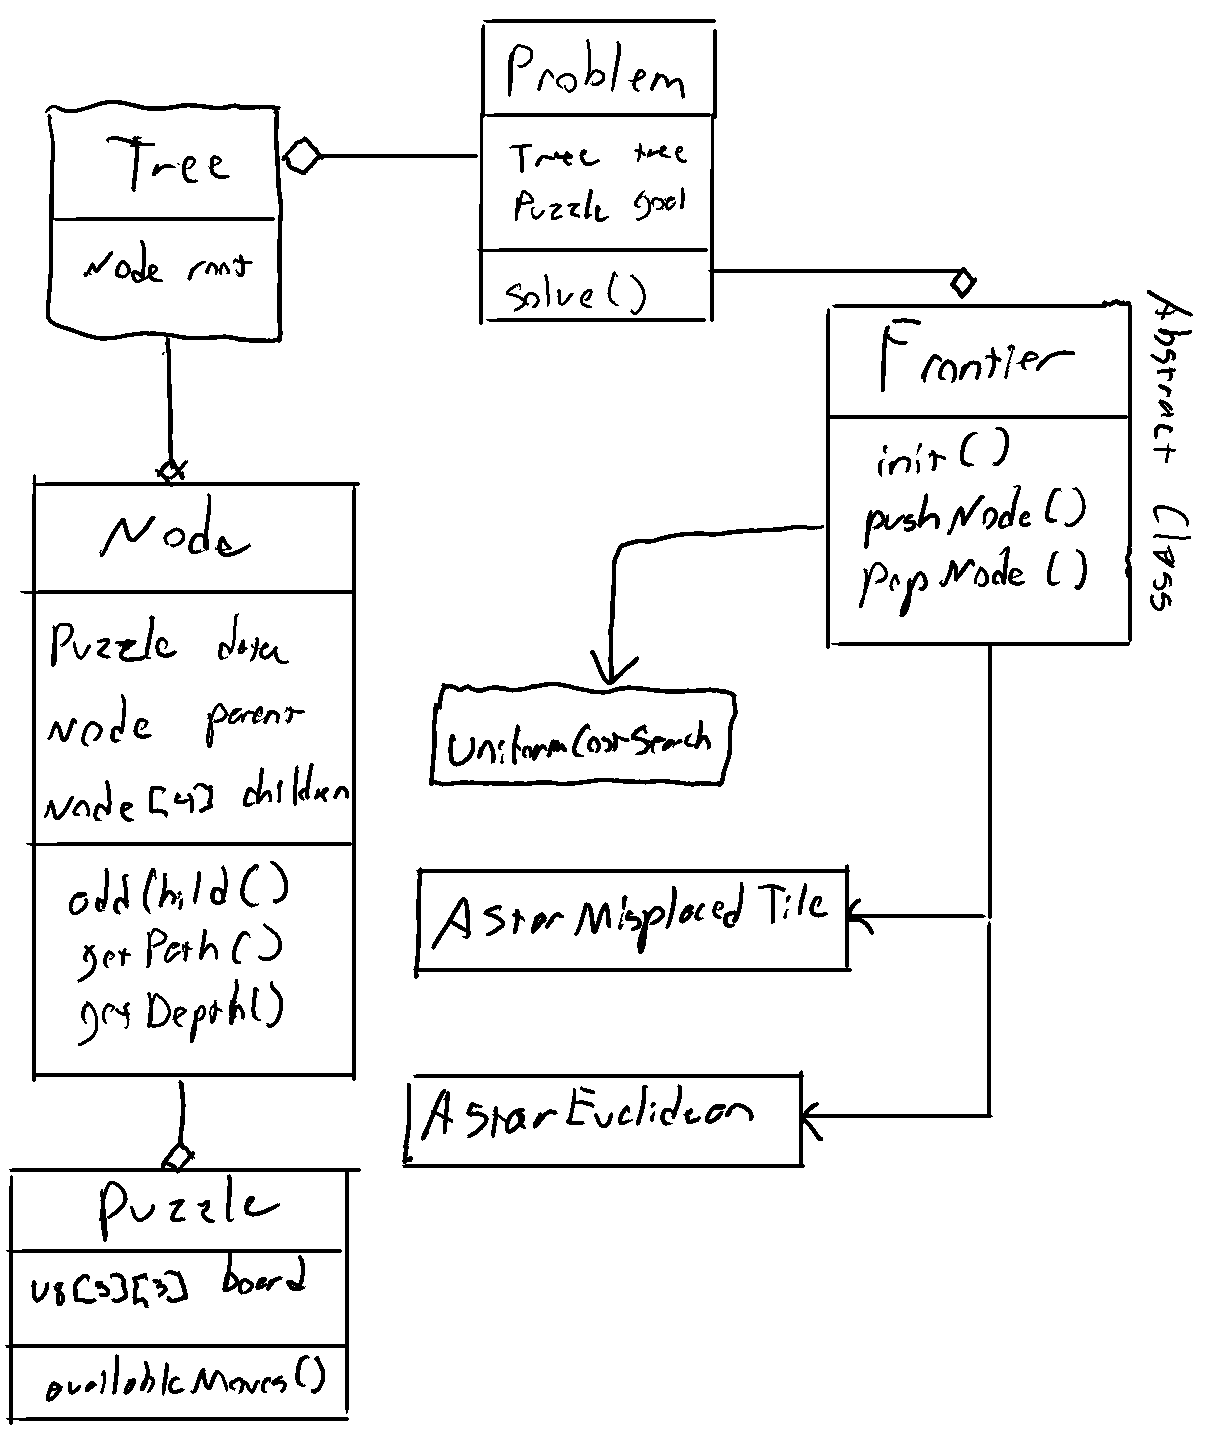
\includegraphics[scale=0.35]{frontier.png}
    \end{center}

    \subsection{Classes}

    \subsubsection{Puzzle --- \texttt{Puzzle.h}}
    The \lstinline|Puzzle| class is the main class that represents the state of the 8-puzzle.
    It is a template class that contains a \lstinline|size_t| template parameter
    \lstinline|N| that represents the width of the puzzle (e.g. 3 for an 8-puzzle).
    The board is represented by a 2D array of \lstinline|uint8_t|.

    The \lstinline|Puzzle| class contains a constructor that takes a 2D array of 
    \lstinline|uint8_t| and performs checks to ensure that the input is valid.
    It also contains an overload for the \lstinline|==| operator to compare two
    \lstinline|Puzzle| states for equality.

    The primary purpose of the \lstinline|Puzzle| class is to generate the next
    possible states from the current state. This is done by the \lstinline|availableMoves|
    method which returns a vector of \lstinline|Puzzle| objects that represent the
    possible states that can be reached from the current state.

    \begin{lstlisting}
        template<size_t N>
        class Puzzle {
        private:
            uint8_t board[N][N];
        public:
            explicit Puzzle(uint8_t board[N][N]);
            std::vector<Puzzle<N>> availableMoves() const;
            bool operator==(const Puzzle<N> &other) const;
        }
    \end{lstlisting}

    \subsubsection{Node \& Tree --- \texttt{Tree.h}}
    The \lstinline|Node| class is a template class that represents a node in the state space tree.
    It contains a \lstinline|Puzzle| state object, a pointer to the parent node, and at most
    4 pointers to child nodes (up, down, left, right).

    The \lstinline|Node| class is designed to be able to reconstruct the solution path
    from the final solved goal state. This is done using the \lstinline|getPath| method
    after the solution has been found.

    The \lstinline|Node| class is the class actually used to build the state space tree
    and perform the search algorithm. The \lstinline|Tree| class is a wrapper around the
    root node of the tree and is held by the \lstinline|Problem| class to keep the memory
    management simple.

    \begin{lstlisting}
        template<class T>
        class Node {
        private:
            T data;
            Node<T> *parent;
            Node<T> *children[4];
            size_t numChildren;
        public:
            Node<T> *addChild(T d);
            std::vector<T> getPath() const;
            size_t getDepth() const;
        }

        template<class T>
        class Tree {
        private:
            Node<T> *root;
        public:
            Node<T> *getRoot();
        }
    \end{lstlisting}

    \subsubsection{Frontier --- \texttt{Frontier.h} \& \texttt{frontiers} directory}
    The \lstinline|Frontier| class is an abstract class that represents a 
    frontier/heuristic for the search algorithm. The \lstinline|Frontier| interface
    contains 2 main methods: \lstinline|pushNode| and \lstinline|popNode|.

    The \lstinline|pushNode| method is used to add a node to the frontier, where
    it will be stored based on the specific implementation of the frontier.
    
    The \lstinline|popNode| method is used to remove and return the next node that
    the search algorithm should expand. The specific implementation of the frontier
    will determine the order in which nodes are popped.

    The \lstinline|frontiers| directory contains the implementations of the different
    frontiers/heuristics that are used in the search algorithm:
    \begin{itemize}
        \item \texttt{BreadthFirstSearch.h} --- Breadth-first search (FIFO)
        \item \texttt{UniformCostSearch.h} --- Uniform-cost search
        \item \texttt{AStarMisplacedTile.h} --- A* search with misplaced tile heuristic
        \item \texttt{AStarEuclidean.h} --- A* search with Euclidean distance heuristic
    \end{itemize}

    Most of the underlying implementations utilize \lstinline|std::push_heap| and \lstinline|std::pop_heap|
    to maintain the queue as a min-heap to optimize the pop time to $O(1)$.

    \begin{lstlisting}
        template<class T>
        class Frontier {
        public:
            virtual void pushNode(Node<T> *node) = 0;
            virtual Node<T> *popNode() = 0;
        }
    \end{lstlisting}

    \subsubsection{Problem --- \texttt{Problem.h}}
    The \lstinline|Problem| class is the driver class for the 8-puzzle solver.
    It contains the code representing the pseudo-code for the Graph Search Algorithm
    within the \lstinline|solve| method.

    The \lstinline|solve| method takes a \lstinline|Frontier| to search with and returns
    a pointer to the goal \lstinline|Node| if a solution is found. If no solution is found,
    the method returns \lstinline|NULL|. The returned \lstinline|Node| can be used to
    reconstruct the solution path using the \lstinline|getPath| method.

    \begin{lstlisting}
        class Problem {
        private:
            Tree<Puzzle<3>> tree;
            Puzzle<3> goal;
        public:
            Problem(Puzzle<3> init, Puzzle<3> goal);
            Node<Puzzle<3>> *solve(
                Frontier<Puzzle<3>> *frontier
            );
        }
    \end{lstlisting}

    \subsection{Compiling \& Running}

    The project is compiled using the \texttt{CMake} utility.
    It requires \texttt{CMake 3.10} or higher and a compiler that supports \texttt{C++17}.

    To compile the project, run the following commands:
    \begin{lstlisting}
        mkdir build
        cd build
        cmake ..
        make
    \end{lstlisting}

    Then to run the project, execute the following command:
    \begin{lstlisting}
        ./CS170Project1
    \end{lstlisting}

    \section{Results}
\end{document}